\documentclass{6033dp1/6033dp1}
\usepackage{graphicx}
\usepackage{enumerate}

\title{CVS: A Collaborative Document Editing System}
\author{Andrew Cooper\\ William Stueck\\ Patrick Vatterott}
\recitation{Recitation 06}

\begin{document}
\maketitle

\section{Introduction}

CVS, named for its creators Cooper, Vatterott, and Stueck, is a peer-to-peer text editing system that avoids the necessity of a central server to host the document. The system is designed to operate in a distributed network where all users are not necessarily connected at any given time. Modifications can be made to the text while a user is not connected to the internet, and once a connection is established, the modifications are applied or merged across all online users. As explained in Section 6.0 below, two users can also synchronize over a local area connection to make real-time updates to the text. 
%\vspace{12 pt} \\

CVS makes use of a sophisticated logging system that keeps track of unique user's modifications to the text. The logging system, accompanied with a text merging algorithm, attempts to automatically merge changes made to the text by the user. If the algorithm detects a conflict that cannot be merged without human deliberation, the users are notified, and the conflicts are resolved manually. CVS also applies different safety mechanisms and data representation techniques to ensure that all users can edit a document seamlessly.

\section{Document Representation}
This section describes how the system design represents a text document and how this design allows the system to detect merging conflicts. The design will use a two-level granularity; the first level represents all of the paragraphs in the document, and the second level represents all of the sentences in the individual paragraphs. By having these two levels, merging conflicts can be examined on a sentence-by-sentence basis. This merging process will be described in more detail in the next section when logging and merging are addressed.
%\vspace{12 pt} \\

The design assumes that every paragraph and every sentence will have a corresponding paragraph and sentence ID. Each paragraph ID will be unique, and each sentence ID will be unique for its corresponding paragraph. This design specification will be accomplished by assigning a masked 32-bit long value to all paragraphs and sentences. The mask will be a 10-bit block corresponding to a unique User ID that will be assigned to each user when the peer-to-peer document is first created. The remaining 22 bits will be assigned when the paragraph or sentence is first created. The mask that is used corresponds to the User ID of the user that initially created the paragraph or sentence.  This masked long value is shown in Figure 1 below.
%\vspace{12 pt} \\

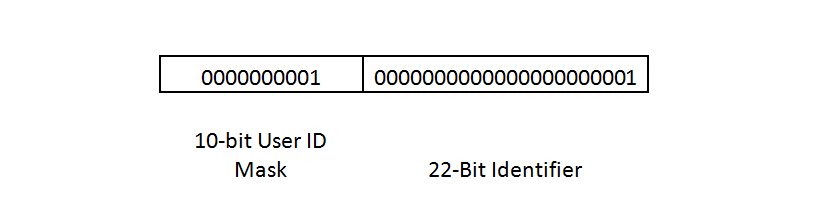
\includegraphics[scale=0.55]{Figure1.png}

The 10-bit mask ensures that every paragraph in the system has a unique ID. The 32-bit ID will be appended to the end of every paragraph in the system but will be unable to be translated by the text editor. This step ensures that the information is stored in the document but is not visible to the user. Within each paragraph, the 10-bit mask will be used to create an ID for each sentence. This 32-bit ID will be appended to the end of the sentence in the document, and just as above, the long value will not be seen by the user. A sample document is shown below in Figure 2.
%\vspace{12 pt} \\

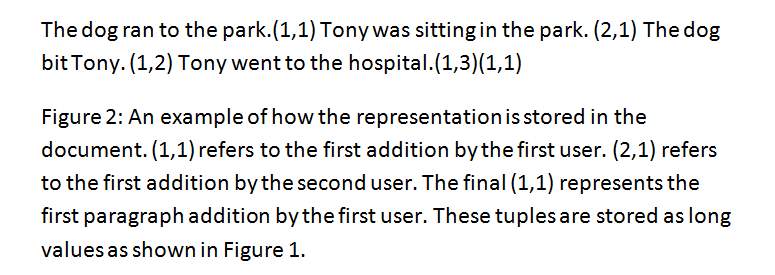
\includegraphics[scale=0.55]{Figure2.png}

The user will never see a document similar to this one because the 32-bit long values will not appear in the actual document, but Figure 2 shows how these IDs will be stored. As you can see, the last sentence has 64 bits appended to it; one for the sentence ID, and one for the paragraph ID.  Finally, the ID of a paragraph or sentence is immutable; it will never change throughout the life of the document.
%\vspace{12 pt} \\

Through this design, a paragraph knows what user it belongs to and its current collection of sentences. A sentence also knows what user it belongs to and can determine its parent paragraph by reading the last appended long value. This information will help the system merge modifications and discover any conflicts that arise due to multi-peer editing.


\section{Tracking Changes}

Each user maintains two data strucutres beyond their document
representation: a change log and a table mapping the other users in 
the group to points in the log. 


\subsection{Log}
As each user edits their local copy of the document, their changes
are continually appended to their local log. The table of commands in
Table \ref{table:log_commands} are appended sequentially to the log as the user edits the in-memory
document. In the table, the symbol \emph{pid} refers to a unique paragraph ID, the symbol \emph{sid}
refers to a unique (within the associated paragraph) sentence ID, and the symbol \emph{uid} refers
to a unique user ID.

%%-------------------------Log Command Table-----------------------------------%%
\begin{table}[h!]
\begin{center}
 \begin{tabular} {|c|c|p{7cm}|}
  \hline
  Log Command & Parameters & Description \\
  \hline \hline
  CREATE\_S & \emph{pid}, \emph{sid} & Created a new sentence with unique ID \emph{sid} in the paragraph with ID \emph{pid} \\
  \hline
  CREATE\_P & \emph{pid} & Created a new paragraph with the unique ID \emph{pid} \\
  \hline
  DELETE\_S & \emph{pid}, \emph{sid} & Deleted the sentence with ID \emph{sid} from the paragraph with ID \emph{pid} \\
  \hline
  DELETE\_P & \emph{pid} & Deleted the paragraph with ID \emph{pid} \\
  \hline
  MOVE\_S & \emph{pid}, \emph{sid}, \emph{pos} & Moved the sentence at (\emph{pid}, \emph{sid}) to position \emph{pos} in paragraph \emph{pid} \\
  \hline
  MOVE\_P & \emph{pid}, \emph{pos} & Moved the paragraph with ID \emph{pid} to position \emph{pos} in the document \\ 
  \hline
  CHANGE\_S & \emph{pid}, \emph{sid}, \emph{string} & Changed the sentence at (\emph{pid}, \emph{sid}) to the text \emph{string} \\
  \hline
  MERGE & \emph{uid} & Merged with the user with ID \emph{uid} at this point in the log \\
  \hline
 \end{tabular}
\end{center}
\caption{The log commands used to track document changes}
\label{table:log_commands}
\end{table}
%%-----------------------------------------------------------------------------%%

\subsection{Checkpoint Table}




\section{Merging}

When two users merge, the user with the higher \emph{uid} is selected to be
the merger. All merging is done on a pairwise basis. If n users are online 
and another comes online, the user with the highest \emph{uid} out of the currently
online group is chosen to do a pairwise merge with the newcomer.

When this happens, the user with the lower \emph{uid} (user A) looks up the last merge point
with the higher \emph{uid} (user B), and sends everything in his log past that point to
A. User B also scans back in the log to the last merge with A and copies this to a new point 
in memory. Using the two differing log parts, User B then resolves conflicts as described below.

When the conflics are resolved, User B appends all of the changes from User A to the end of his log
and applies them to his working copy. He sends the portion of his log after the previous merge with
A to A, and appends a "MERGE A" to the end of his log.

When User A receives the new log from B, he rolls back all of his changes so that his document appears
as it did at the last merge with B. He then applies the new changes from B and replaces his portion
of the log since the last merge with the resolved log.

\subsection{Conflict Definitiion}
With the current log representation, there are a number of conflicts that need to be resolved manually
by the merging user. These conflicts are:

\begin{enumerate}[1)]
\item The two users change the same sentence in different ways. A deletion is considered a change.

\item The two users move a sentence to different locations.

\item The two users move a paragraph to different locations.

\item One user deletes a paragraph, another edits its contents (changes a sentence).

\item One user deletes a sentence, another changes it.

\end{enumerate}

These are not considered conflicts, and will be ignored:

\begin{enumerate}[A)]
\item The two users change a sentence to the same thing.

\item The two users move a sentence to the same location.

\item The two users move a paragraph to the same location.

\item The two users delete the same sentence/paragraph

\item One user edits a paragraph, one moves it.
\end{enumerate}

\subsection{Conflict Resolution Algorithm}
This algorithm identifies conflicts and presents them to the user for resolution.
It takes as arguments two log file parts from different users.

The algorithm works by traversing the two log parts backwards (from most recent change
to oldest change) and determining if the most recent changes to each paragraph and sentence
conflict between the two log parts. This is accomplished by first traversing backwards
through the log of the merging user and building up two tables. These tables look like this:

%%-------------------------Paragraph Table-----------------------------------%%
\begin{table}[h!]
\begin{center}
 \begin{tabular} {|l|l|l|l|l|}
  \hline
   \emph{pid} & Modified & Deleted & Moved & New Location \\
  \hline \hline
    421 & 1 & 1 & 0 & 0 \\
   \hline
    512 & 0 & 0 & 1 & 421 \\
   \hline
    21 & 1 & 0 & 0 & 0 \\
   \hline
    893 & 1 & 0 & 0 & 0 \\
   \hline
 \end{tabular}
\end{center}
\caption{Table tracking changes to paragraphs}
\label{table:paragraph_table}
\end{table}
%%-----------------------------------------------------------------------------%%

Table \ref{table:paragraph_table} (above) shows the table used for tracking paragraph
changes. Table \ref{table:sentence_table} (below) shows the table used for tracking
sentence changes. Both are built dynamically, there are not entries for each paragraph
and sentence when they are created. 

%%-------------------------Sentence Table-----------------------------------%%
\begin{table}[h!]
\begin{center}
 \begin{tabular} {|l|l|l|l|l|l|}
  \hline
   (\emph{pid}, \emph{sid}) & Modified & New Content & Deleted & Moved & New Location \\
  \hline \hline
    (421, 75) & 1 & "New Sentence" & 0 & 0 & 0 \\
   \hline
    (512, 32) & 1 & NULL & 1 & 0 & 0 \\
   \hline
    (21, 88) & 0 & NULL & 1 & 0 & 0 \\
   \hline
    (21, 99) & 0 & NULL & 0 & 1 & 34 \\
   \hline
 \end{tabular}
\end{center}
\caption{Table tracking changes to sentences}
\label{table:sentence_table}
\end{table}
%%-----------------------------------------------------------------------------%%

These tables track certain characteristics useful in conflict resolution. The algorithm
then traverses the imported log part in a backwards manner, following these rules:

\begin{enumerate}[1)]

\item When encountering a DELETE\_P, if the modified bit is set in the paragraph table for this paragraph,
      there is a conflict and the user is prompted. If the user keeps the deletion, the
      statement remains in the log, otherwise it is removed.

\item When encountering a DELETE\_S, if the modified bit is set in the sentence table for this sentence,
      there is a conflict and the user is prompted. If the user keeps the deletion, the
      statement remains in the log, otherwise it is removed.

\item When encountering a CHANGE\_S, if the most recent change to a sentence changes it to different text
      than is recorded in the table, prompt the user to fix the conflict. If they choose the local sentence,
      or the most recent change is the same as what as in the table, delete this and all previous chanes
      to this sentence in the foreign log. If they choose the foreign sentence, delete changes in the 
      local log.

\item When encountering a MOVE\_P, if the moved bit is set in the paragraph table for this paragraph,
      check if the targets are the same. If they are different, prompt the
      user to resolve the conflict. If he chooses the local version, or the targets were the same, 
      delete all moves to this paragraph
      from the foreign log part. If he chooses the foreign version, delete all moves to this paragraph
      from the local log part.

\item When encountering a MOVE\_S, if the moved bit is set in the sentence table for this sentence,
      check if the targets are the same. If they are different, prompt the
      user to resolve the conflict. If he chooses the local version, or the targets were the same, 
      delete all moves to this sentence 
      from the foreign log part. If he chooses the foreign version, delete all moves to this sentence 
      from the local log part.

\item Keep all MERGE and CREATE statements in the log.
\end{enumerate}

\subsection{No Conflict Example}


\subsection{Conflict Example}










\section{Commit Points}

A commit point is defined as a point in time when a user can manually commit the current version of the document, and once every user agrees on the commit, that current state of the document is preserved on all systems.  This functionality allows users to save previous versions of a file and also allows them to have a file backup in the event of a system crash.
%\vspace{12 pt} \\

The design requires that every user be online before a commit can be made. This requirement makes sure that every user agrees to the commit point and that all outstanding modifications and conflicts are merged correctly. In order to merge, a user's log file must be completely caught up with every user in the system. If the user's last log entry contains sync pointers to every user in the system, then the user will be allowed to issue a commit. The commit process is described below.
%\vspace{12 pt} \\

After a user is completely up to date with all other online users and the commit is issued, the committing user queries all other users. This query simply asks if the queried user is in accordance with the commit point. If a user is not in accordance, then the commit fails, and that information is returned to the committing user. If all users are in accordance, the query returns "True" to the committing user. When "True" is returned, the current version of the file is saved to every user's system in the current working directory.  Assuming the original document is named \emph{original.txt}, the file saved onto each system will be \emph{original\_commitName.txt}, where \emph{commitName} is the name the committing user assigned to the commit. Given $n$ commits of a document, the working directory should contain $n+ 1$ documents; one original document and n committed documents.

\section{Synchronization}

Synchronization occurs when two users connect their computers over a local area connection, i.e. an Ethernet cord or shared WIFI. When two users are synchronized, each user can make updates to the document that are then immediately visible to the other user.  These users can then acquire an internet connection and merge documents with a third party just as before.
%\vspace{12 pt} \\

The major problem with synchronization is the conflict that arises when two users are simultaneously trying to modify the same" part" of a document. In this sense, "part" refers to the sentence level of granularity in the system design. To address this problem, the design uses a locking system to protect a sentence from being modified at the same point in time.
%\vspace{12 pt} \\

 When a user places the cursor in a particular sentence in the document, the P2P system first grabs the 32-bit ID of the sentence. This ID is relayed to the other user currently in synchronization. That user's system locates the sentence and locks it; the user is unable to place a cursor within that sentence. Once the editing user moves to a different part of the document, an unlock signal is sent to the other user. This system prevents simultaneous editing of the same sentence.
%\vspace{12 pt} \\

During this locking and unlocking process, the two users share a central log file. Every modification made by either user is appended to the log file. The locking system prevents merging conflicts, so one log file is safe to use. When synchronization is over, this central log file is appended to the end of each user's log file that existed before synchronization. A pointer to the opposite user is placed at the last entry, and the log file is then up-to-date and correct. Merging between a third party can then be handled using the normal method described above. 

\section{Analysis}

CVS must be performance analyzed from three perspectives to fully understand the quality and limitations of the system.  First, CVS must be scalability analyzed to see how large the system can get in terms of users as well as file size.  CVS must then be analyzed for performance in terms of the space requirements as well as runtime requirements.

\subsection{Scalability Limits}

CVS puts an upper bound on the number of users that can use the system.  In order to label each sentence and paragraph with a 32-bit integer, CVS chooses to allocate 10 bits to identifying the user responsible for creating the sentence or paragraph, and the remaining 22 bits are for identifying the sentence or paragraph.  As a result, CVS supports at most 1,024 users, and each user can create at most approximately 4 million paragraphs.  Each paragraph can contain at most approximately 4 million sentences.  See Figure 3 for details.

\begin{figure}
\begin{center}
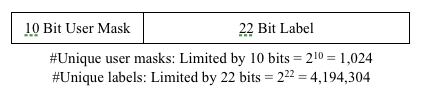
\includegraphics[scale=0.55]{analysis_figure_1.png}
\end{center}
\caption{Shows the structure of a sentence label as well as the arithmetic used to calculate the maximum number of users, sentences, and paragraphs.}
\end{figure}

\subsection{Space Analysis}

CVS requires space in implementation beyond the space necessary for storing the document for 3 reasons.  First, the system needs space to label each part of the document.  Then, the system needs to maintain a log of changes made.  Finally, the system needs to keep a table to track the locations of pointers for each checkpoint within the log.

\subsubsection{Labeling Overhead}

As noted above, labeling parts of the document will increase the length of the document by 32 bits for each sentence as well as 32 bits per paragraph.  Encoding each character using Unicode allocates 16 bits to each character.  Therefore each label effectively adds two characters, 32 bits, to the document.  Assuming the average paragraph has 10 sentences, CVS's labeling system effectively adds 22 characters per paragraph.  Since a paragraph has 872 characters on average, CVS labeling causes space overhead of 2.52\%.  See Figure 4 for details.

\begin{figure}
\begin{center}
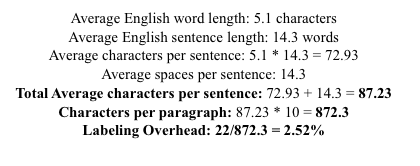
\includegraphics[scale=0.55]{analysis_figure_2.png}
\end{center}
\caption{Shows the arithmetic for calculating the labeling overhead.}
\end{figure}



\subsubsection{Logging Overhead}

As noted in Design, the log file holds information about how the file has changed since the last commit.  In the worst case, a user has changed every single sentence since the last commit.  This means that there is an entry in the log for each sentence.  Since a log entry is for all intents and purposes a sentence itself, the log is the size of the original file in the worst case.  In reality, the log is likely to be much smaller than the original file, but the space used has as upper bound the size of original file.

\subsubsection{Checkpoint Table Overhead}

As described in Design, CVS maintains a table with pointers to the location in the log where each of the last checkpoints was made with each user.  Therefore, the table with have one entry for each user, with one piece of data for each user (the pointer).  If the system has m users, there will be $2*m$ entries in the log.  This will be significantly smaller than the document itself or the log, so it is negligible.




\subsection{Runtime Analysis}

CVS has one main computationally intensive process: that of merging documents.

\subsubsection{Merging Runtime Analysis}

When two files merge, two processes must happen.  First, the program must determine where there are potential conflicts.  Then, the program must determine if a conflict actually exists.  All locations where a conflict exists are locations that the user must resolve himself.  Assume that the document has m sentences.  In the worst case, both users have changed all m sentences.  This means that each log has m entries.  In order to determine locations for potential conflicts, the merge table, as described in Design, is created based on one user's log.  The other user's log is then compared to this table to locate possible conflict sentences.  This amounts to $m^2$ comparrisons in the worst case, as each time a conflict is found, the algorithm deletes all changes from the log that led to the conflict as part of the garbage collection process.  In other words, the log must be traced through $m$ entries, and for each entry, there are $m$ possible log items that may need to be deleted.  Since the document has only $m$ sentences, only $m$ conflicts must actually exist.  In order to test for conflict, the system must compare characters in each sentence.  Since a sentence has approximately 87 characters on average (see Figure 3), this amounts to $87*m$ operations.  That way, merging takes $m^2 + 87*m$ operations in the worst case.  This is not unreasonable.  If we assume that a document has 10,000 sentences, which is an extreme case, as we expect documents to be smaller than this, merging will take 100,870,000 operations.  On a modern processor that can do 109 operations per second, that merge will take only 0.1 seconds.  See Figure 5.

\begin{figure}
\begin{center}
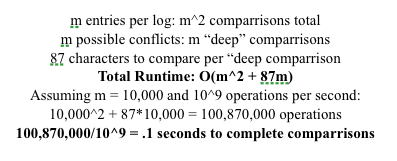
\includegraphics[scale=0.55]{analysis_figure_3.png}
\end{center}
\caption{Shows the runtime analysis of merge, as well as the arithmetic to determine the time in seconds.}
\end{figure}


\section{Conclusion}

CVS successfully handles all requirements and scenarios posed in the Design Project 2.  CVS does this with limited space and runtime resources, which make the system an excellent option for users looking for a quality peer to peer collaborative document editing system.  The system does have some limitations, as noted in the design and analysis, but these limitations are extreme edge cases and are unlikely to ever affect the actual user.  Moving forward, we would like to open source CVS, which will allow users to optimize the system for their own needs and will allow the most users possible to benefit from CVS.

\section{Word Count}
4277



\end{document}
